\section{\toolname: System Design}
\label{sec:systemDesign}

\begin{figure*}[t]
 \centering
 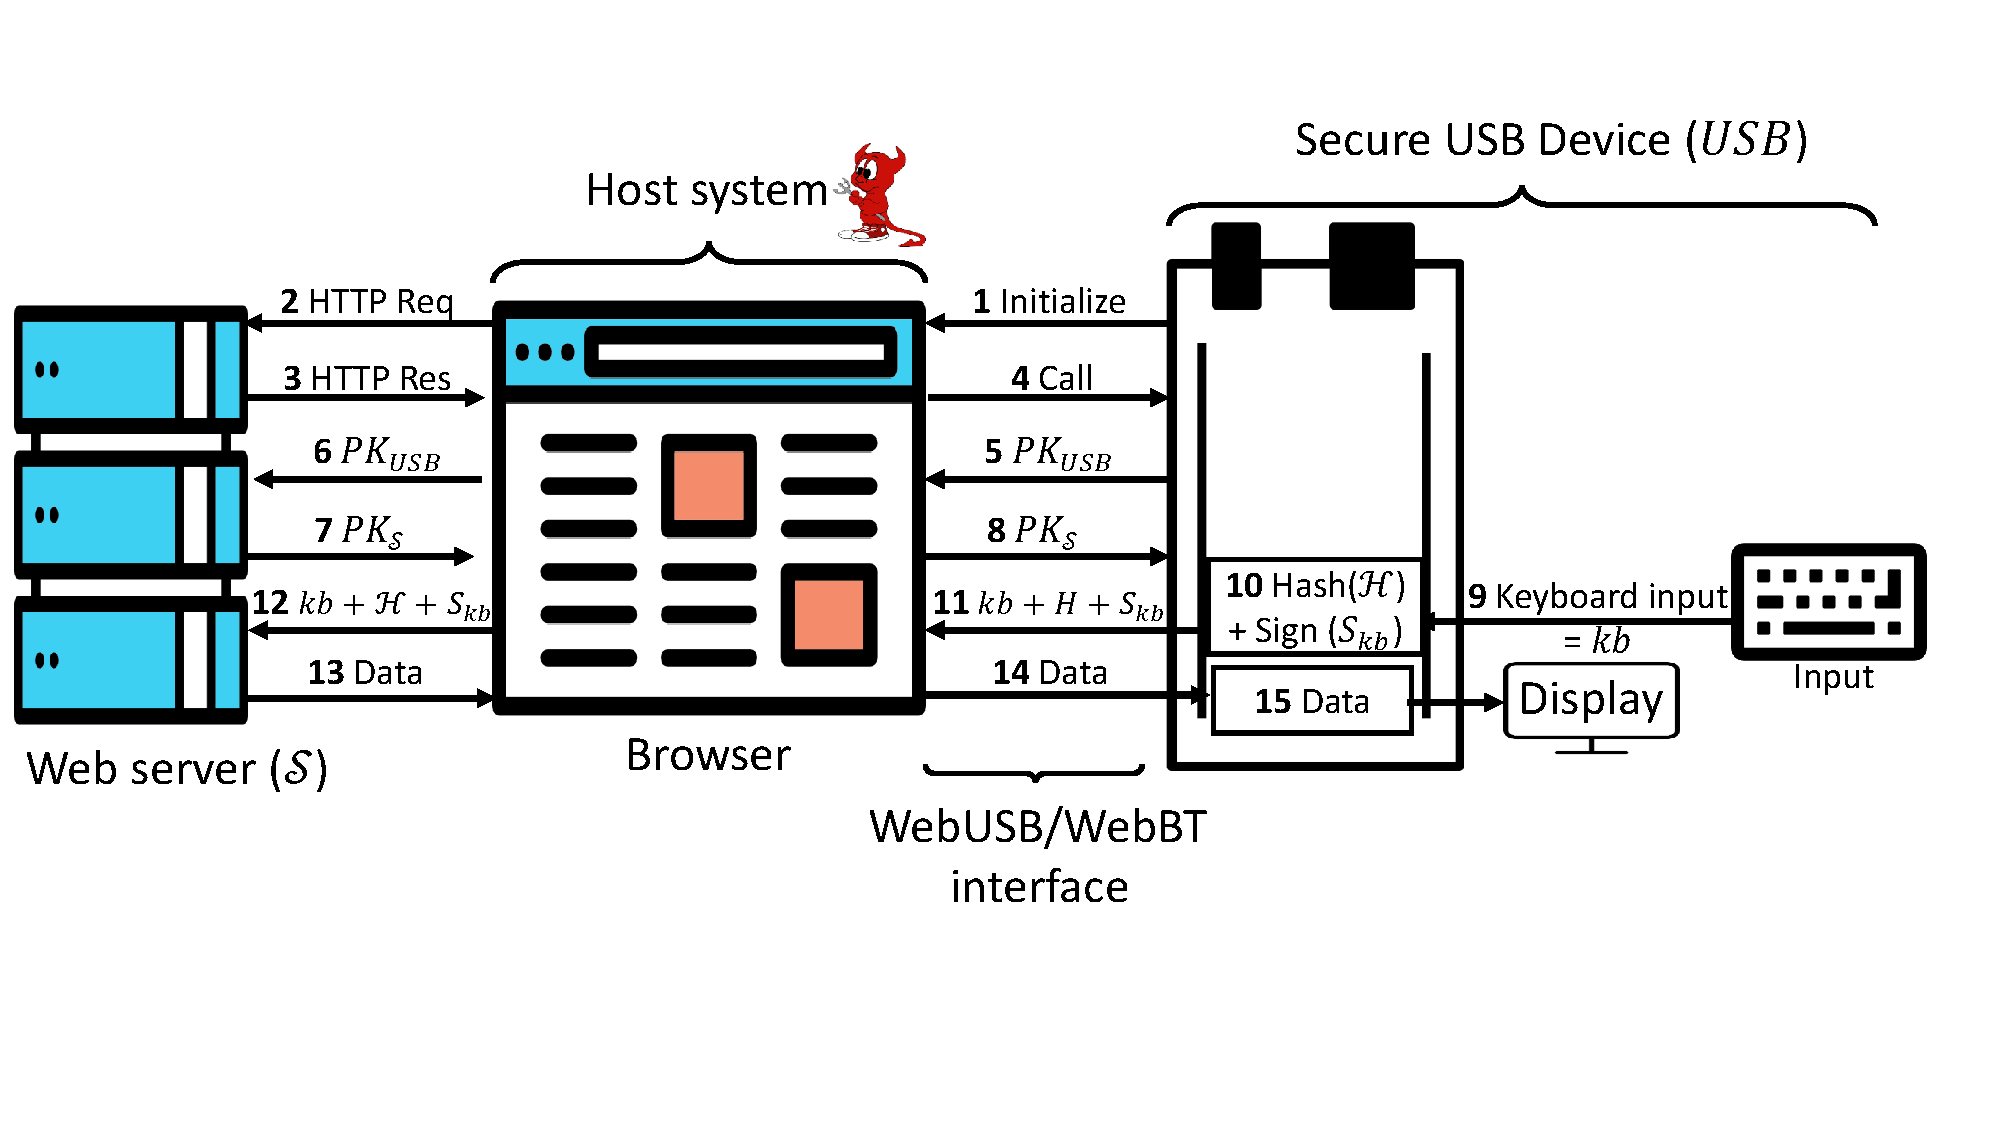
\includegraphics[trim={0 3cm 1cm 1cm}, clip, width=\linewidth]{SystemDesign_auth_ip.pdf}
 \caption{System design of \tool. The diagram provides the interaction between the components in the system and the messages that are exchanged between them to establish a secure channel from the \device to the remote server (\server). Steps $1-4$ denotes how the user loads a web page from \server that serves a \js snippet. The \js snippet is written using the \webusb/\webbt API. Steps $5-8$ shows the establishment of the \tls channel using the browser as an untrusted transport. $PK_{USB}$ and $PK_{\mathcal{S}}$ are the public key corresponding to the \device and \server respectively. We assume that \server is trusted and there exists a PKI that we can leverage, Using the PKI, the \device verifies \server's public certificate. Steps $9-12$ shows how the user types a message on the input peripherals that are connected to the \device that transfers the keystrokes securely to \server along with the signature to ensure integrity and authenticity of that input. The \device also houses a primitive display that shows useful information such as the certificate information of \server and confirmation/information related to the service the user is using.}
 \label{fig:systemDesignAuthInput}
\end{figure*}

Our proposed solution preserves input integrity, authenticity, and confidentiality by extending a secure channel (\tls) to an independent trusted embedded device. We call this device ``\device'' and it leverages the \webusb API provided by the browser to connect to a remote web server (we denote this remote server as \server). The \tls channel initialized by the \device is secure against the malicious operating system and the browser. We assume that the attacker can compromise the host system hardware, operating system, and installed applications. 

\myparagraph{\webusb.} We leverage \webusb for the communication between the \device and the trusted remote server (\server). \webusb is an upcoming standard in development~\footnote{Protocol description is located at \url{https://wicg.github.io/webusb/}} by Google and currently implemented as an experimental feature in the Google Chrome web browser. \webusb allows a \js code served from a \https secured page to have direct access to the \usb device. The \webusb API allows the web-pages to enumerate and communicate with the \usb devices attached to the host system, provided that the proper \usb driver is installed in the operating system.


\subsection{System model} 
\label{sec:inputPrivacy:systemModel}
Our system model primarily involves four components. The \usb/\bluetooth enabled peripheral (keyboard, mice, bulk storage or any peripheral devices), a host which is a computer/smartphone that connects to the remote server using a web browser, the aforementioned remote server where the host is connected to and lastly the \device that converts any generic \usb/\bluetooth peripherals to secure peripheral. The general setting assumes that the peripherals are connected to the \device and the \device is connected to the host system. The connection could be wired or wireless depending on the case if the host system is a computer or a smartphone. Similarly, the communication between the \device and the input peripherals can be carried out by wired or wireless channel depending on the nature of the peripherals. The system model is independent of the physical connection between the host, \device and the peripherals. 
%Our designed \device is a small embedded device with very small TCB (few thousand lines of code) yet computationally powerful to carry out cryptographic operation efficiently.

\subsection{Secure Channel Establishment}
\label{sec:systemDesign:secureChannel}

We assume that the remote server \server is a trusted entity and has a public certificate and corresponding public-private key pair to prove its authenticity by leveraging some existing PKI. \server serves a \js snippet that uses \webusb API to communicate with the \device. The \device has a long-term key-pair ($PK_{usb}, SK_{usb}$) embedded that is used to establish a secure channel (\tls) with \server. The user attaches all her USB peripheral devices with the device to eliminate any input manipulation or forged data generated by the malicious host. Figure~\ref{fig:systemDesignAuthInput} provides the overall system design of our system. It shows all the components of the systems and abstracts all the messages exchanged between them. The flow of the system is as follows: 

\iffalse
\paragraph{Initialization} The user initializes the device by providing a domain name and coupling the credential corresponding to the domain. One such example is: the domain \server $=$ \texttt{xyz.com} and the credential \credential $=$ \texttt{(username, password)} where the tuple corresponds to the username and the password. The device uses a cryptographic hash  function to hash the credential and generates $\mathcal{H}_{\mathcal{S}} \leftarrow HASH$(\credential).
\fi

\begin{enumerate}
  \item The user types a specific address \server\ in the browser. As the input peripherals (e.g., keyboard) are connected to the \device, it can record the web address the user provides.
  
  \item When the web page from the address \server\ is loaded, the \device communicates with \server directly via \webusb\ API.
  
  \item \server and the \device then establishes a secure channel (\tls) using their long-term key pairs. Over this secure channel, the device requests \server's certificate information along with a challenge (nonce) for freshness.
  
  \item Upon receiving the request, \server sends the certificate along with the nonce and signs the entire message with its private key. Upon receiving the certificate, the \device verifies it.
  
  %\item If the certificate information and the signed nonce are correct, the device shows a security indicator which identifies the web server as the legitimate one. Otherwise, it raises an alarm to notify the user about a potential attack.

\end{enumerate}  

After a secure channel is established, the device uses the session keys to sign each input data. %Alternatively, it can also use the session secret to encrypt keystrokes to the remote server, so any other party except the remote server can not decrypt the messages in any meaningful way. 
As all the messages are accompanied by the digital signature, anyone other than the specific \device can not forge messages.


\begin{figure*}[t]
 \centering
 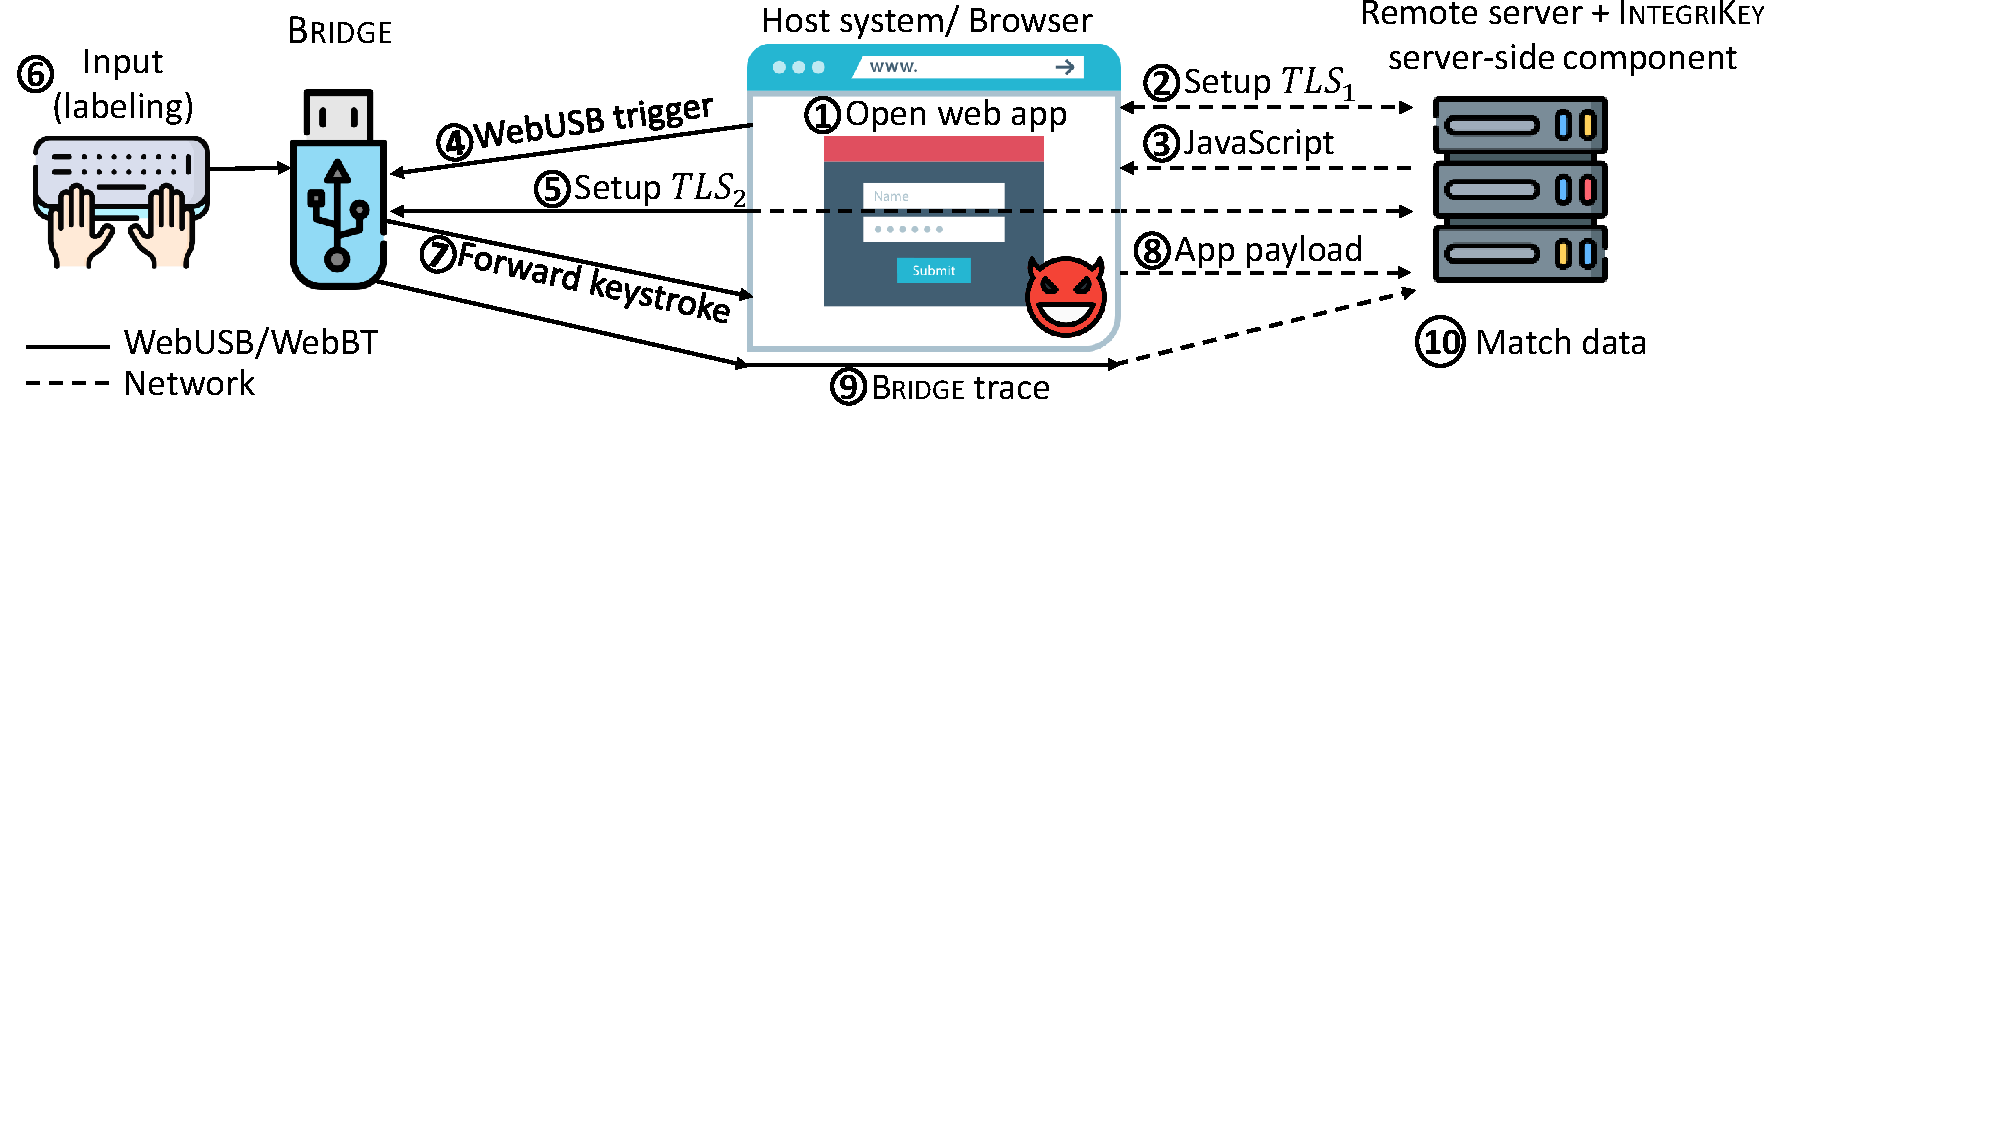
\includegraphics[trim={0 6cm 3cm 1cm},clip,width=\linewidth]{SystemDesign_forms.pdf}
 \caption{System design of our proposed solution to provide integrity protection for input data. One such use case is filling up text fields in the browser. We assume that the \device already established a secure channel (\tls) with the remote server (\server) (as explained in Section~\ref{sec:systemDesign:secureChannel}). Steps 1-5 shows that the user provides the input through the keyboard which is connected with the \device. The \device computes the cryptographic hash of the input data and compute digital signature on the hash value. The \device sends the input data to the \server. Upon receiving, \server computes the hash over the submitted data (step 6). Then in step 7, the \device sends the previously computed hash and the digital signature to \server via the dedicated \tls channel (step 8 and the dotted line). Finally \server checks the hash competed by itself (step 6) and the received hash in step 9. Additional \server also verifies the signature to determine authenticity of the data.}
 \label{fig:systemDesignForms}
\end{figure*}

 
\subsection{Authenticity of the Input Data}
\label{sec:systemDesign:integrityVerification}

Our solution enables the verification of the input data provided by the user in cases where privacy of the input data is not concerned, but only the integrity and the authenticity of the data. One such example is the banking transaction where the user needs to fill several input textfields such as the beneficiary name, account number, address and the amount of money to send. A malicious host can either manipulate some of the input fields or generate some false data. Such as, changes in the amount of money or the destination account number. Such modifications can be hidden from the user completely as the browser never changes the graphical elements (such as the \texttt{inputTextField.value}) but changes the data in the web request (\texttt{HTTP} payload) before sending it to the remote server. We eliminate this problem using the following steps, detailed interaction diagram is provided in Figure~\ref{fig:systemDesignForms}.

\begin{enumerate}
  \item After the establishment of the secure channel (\tls) between the \device and the remote server (described in Section~\ref{sec:systemDesign:secureChannel}), the server sends a webpage containing the input forms. The \device also requests the web server via the dedicated secure channel, the identifiers of the input field on the current page.
  \item When the user provides the input ($data$) to the form via the device the device stores the input to its memory and passes it on to the browser.
  \item When the user sends the form, the device calculates a set of cryptographic hashes $\mathcal{H} = \{\mathcal{H}_1, \mathcal{H}_2, \ldots, \mathcal{H}_n\}$ and digital signatures $\mathcal{SG} = \{\mathcal{SG}_1, \mathcal{SG}_2, \ldots, \mathcal{SG}_n$)\} corresponding to the input field data $d_1, d_2, \ldots, d_n$. 
  $$\mathcal{H}_i \leftarrow Hash(d_i),\ \mathcal{SG}_i\leftarrow Sign_{{SK}_\texttt{USB}}(\mathcal{H}_i)$$
  where ${SK}_\texttt{USB}$ is the private key of the \device. 
  \item The \device then sends $\mathcal{H}$ and $\mathcal{HG}$ to the remote server \server. Upon receiving, \server verifies the signatures and accepts if all the signatures are correct corresponding to the cryptographic hash of the input data. 
\end{enumerate}

\subsubsection{Detailed message structure}

Here we specify the message structure of the \device when it sends the authenticated keystrokes to the remote server (\server). We assume that the long-term public-private key pairs of \server and the \device is $\{PK_\mathcal{S}, SK_\mathcal{S}\}$ and $\{PK_\usb, SK_\usb\}$ respectively. Assume $k_{\mathcal{S}, \usb}$ is the session key established between \server and the \device and $T$ is the session token established in the \tls session which is unique for a specific \device. The \device construct the following message blob $MB$ for a keystroke message $KS$ where

\[
  MB \leftarrow 
    \underbrace{Hash (KS)}_{\text{Hashed Message = $\mathcal{H}$}} \| 
    \underbrace{TS}_\text{Timestamp} \|
    \underbrace{Sign_{SK_\usb}(T| \mathcal{S}| \mathcal{H} | TS)}_\text{Signature}
\]

A keystroke message $KS$ is defined as the concatenation of the input field ID and the actual data that the user provides from the input device via the \device.  When the user selects a textfield, the \js code fires an \texttt{onSelect()} event that notifies the server and the \device about the textfield that is selected by the user.
\[
    KS \leftarrow  \underbrace{(id_i\|data_i)}_{\text{for input field $i$}}
\]

 
\subsection{Protection against Swapping of Input Fields}
\label{sec:secureChannel:swappingFields}

A more sophisticated version of the attack described in the previous section (\ref{sec:systemDesign:integrityVerification}) can be orchestrated by a malicious host where it can swap various input fields on the webpage. Here the individual input data is not manipulated, but the user is tricked into putting data in the wrong fields. One concrete example is the web interface to change the parameters of a pacemaker device. Many of the parameters' data type can be identical (such as numbers) but interchanging the actual values may be life-threatening. To prevent such an attack, we propose a mechanism for the \device to communicate with the remote server and bind input data to the label of input. There are two parts to this proposed solution, one of them is executed on \server and another on the \device at the user side.

\subsubsection{Server side computation}

 We develop a framework that can take any arbitrary web page, parse it and extract the input fields from there. The framework then calculates the set of fields that are potentially interchangeable. We assume that the logic in \server already employs some filters that eliminate wrongly formatted data. This is why we focus more on the similar fields which are very hard for \server to distinguish and prevent the input field swapping attack. The framework parses the web page and infers the data type (such as \integer, \float, \String, \boolean etc.) of every field. Additionally, the developers can provide more fine-grained details such as the range of values (in case it is a number datatype), possible minimum and maximum length, the regular expressions for the \String-typed data etc. From this details, the framework creates a set for groups: $G_1, G_2, \ldots, G_n$ where each group contains a set of fields which are potentially interchangeable. One example is field $F_1$ and $F_2$ both of which are numerical fields. We assume $F^{max}$ and $F^{min}$ denote to the maximum and minimum possible values corresponding to the field $F$. If one the following conditions holds:
 
$$F_1^{max} < F_2^{min} \ \text{or}\ F_1^{min} > F_2^{max}$$ 

then there exist no overlapping values that can be the valid inputs to either $F_1$ or $F_2$ or both, otherwise, the framework outputs $G=\{F_1, F_2\}$ as a group of fields which can be swapped by a malicious host system.

Additionally, the framework executes analysis on various data types. The analysis requires a specification from the developers that describes the characteristics of the input fields. This specification may contain a \String regular expression. The framework contains a knowledge database that specifies the regular expression for the well-known fields. One such example is the name is an alphabetic type and can be represented as $s[a-zA-Z]^+[\_]^*[min=1, max>min]$. The address is an alphanumerical \String datatype and can be represented as $s[a-zA-Z]^+[0-9]*[\_]^*[min=10, max>min]$. 

The format of the specification is the following

$$datype[regx][min = x, max = y]$$
The $datatype$ denotes the input datatype such as \String($s$), \integer($i$), \float($f$) and \boolean ($b$). $[regx]$ is valid only for the \String datatype. $min$ and $max$ represents the minimum and maximum length of the data respectively if the datatype is \String, minimum and maximum value of the data if the datatype if \integer or \float. Upon feeding all the specification to the framework, the framework evaluates all the input field by executing a membership test. The test to find the overlapping values for the \integer and the \float type is discussed above. For the \String datatype, the test involves membership criteria, i.e.,

\[s[a-zA-Z]^+[\_]^*[min=x, max=y] (=RE_1)\subset\] 
\[
s[a-zA-Z]^+[0-9]^*[\_]^*[min=x, max=y] (=RE_2)
\]

which can be verified by checking the following conditions:

\[
(RE_1\cap (RE_2)^c = \phi) \wedge (RE_1.max < RE_2.min \vee RE_1.min > RE_2.max)^c
\]

The subset criteria may also change depending on the minimum and maximum length of the specific input fields. There could be two cases where field interchange may happen:
\begin{enumerate}
  \item \textbf{Fully interchangeable:} This can happen if the regular expressions corresponding fields $F_1$ and $F_2$ satisfy the following condition
  \[
  (re_1 \subset re_2 \wedge re_2 \subset re_1) \wedge (RE_1.max = RE_2.max \wedge RE_1.max = RE_2.max) 
  \]
  \[
  \implies  re_1 = re_2
  \]

  \item \textbf{Partially interchangeable:} Where one field's regular expression is a subset of another field. E.g., if $re_1 \subset re_2$ then the data of $re_1$ can replace $re_2$ as all possible values of $re_1$ can be valid input to $re_2$ but the reveres is not true.  
\end{enumerate}

\server sends this information to the \device when the user loads a specific web page containing the input fields.

\lstset{language=XML, caption=Specification of the input fields by the developers, label = snippet:specificationXML, firstnumber =1}
\begin{figure}[t]
\begin{lstlisting}[mathescape=true]
<InputSchema>
 <Input>
   <Type>"String"</Type>
   <Tag>Relay 1</Tag>
   <RegEx>"s[a-zA-Z0-9]+[\_]*[min=1, max>min]"</RegEx>
   <Max>x</Max>
   <Min>y</Min>
 </Input>
 <Input>
   <Type>"String"</Type>
   <Tag>Relay 2</Tag>
   <RegEx>"s[a-zA-Z0-9]+[\_]*[min=1, max>min]"</RegEx>
   <Max>x</Max>
   <Min>y</Min>
 </Input>
 <Input>
   <Type>"Integer"</Type>
   <Tag>Temp Relay 1 (deg c)</Tag>
   <RegEx>"i[0-9]*[min=-20, max=150]"</RegEx>
   <Max>x</Max>
   <Min>y</Min>
 </Input>
 <Input>
   <Type>"Integer"</Type>
   <Tag>Temp Relay 2 (deg c)</Tag>
   <RegEx>"i[0-9]*[min=-10, max=100]"</RegEx>
   <Max>x</Max>
   <Min>y</Min>
 </Input>
</InputSchema>
\end{lstlisting} 
\end{figure}

\subsubsection{Client side computation}

\begin{enumerate}
  \item As described in Section~\ref{sec:systemDesign:secureChannel}, the server \server\ and the \device establish a secure channel (\tls) leveraging the \webusb\ API.
 
  \item \server sends the web page containing the form to the browser. When the user fills up the form, he also puts the identifier of the field (the title) at the beginning of the field.
  
  \item The \device calculates the cryptographic hash of the fields ($\mathcal{H}$) and the digital signature of the fields ($\mathcal{SG}$).
  We assume the form with input fields $F_1, F_2, \ldots, F_n$ contain the identifiers $id_1, id_2, \ldots, id_n$. The user fills the form as $\mathcal{D} = id_1\|d_1, id_2\|d_2, \ldots, id_n\|d_n$ where $d_i$ is the input data corresponding to the field $f_i$ and ``$\|$'' represents \String concatenation.
  $$\mathcal{H} \leftarrow Hash(\mathcal{D}),\ \mathcal{SG} \leftarrow Sign_{{SK}_\texttt{USB}}(\mathcal{H})$$ 
  where $SK_\texttt{USB}$ is the private key of the \device.
  \item The \device then sends $\mathcal{D}$, $\mathcal{H}$ and $\mathcal{SG}$ to \server.
  
  \item Upon receiving $\mathcal{D}$, $\mathcal{H}$ and $\mathcal{SG}$, the server checks the identifier of the data from the fields if they are valid, checks the cryptographic hash and the digital signature. This way we make sure that even if the malicious host swaps the fields, it can not send wrong data to the server as the data is associated with the identifier of the field provided by the user.

\end{enumerate}



\ifpaper

\subsection{Eliminating User Credential}
\label{sec:systemDesign::passwordManager}

We extend the idea of preserving the integrity and authenticity of the user's input to strong server authentication.
We propose a method to use the \device as a dedicated hardware backed credential manager that eliminates the need for the user to provide the credential through the web application. As we discuss in the Section~\ref{sec:systemDesign:secureChannel}, the \device establishes a secure channel (\tls) with the trusted remote server using the \webusb API.Upon successful establishment of the secure channel, the \device transfers the credential to the remote server directly. Thus eliminating any possibility of the compromised host system to manipulate or steal the sensitive credential. The proposed method ensures dispatch of the credential if and only if the remote server successfully proves its identity. This ensures that the malicious host cannot fake a web application to prompt the user giving the credential. 

\iffalse 
We extend the idea of protecting the integrity of the input data and strong server authentication to use the \device as a dedicated hardware backed password manager. This provides protection against phishing website that tracks the users into leaking their credentials. The device prevents thing by establishing secure channel using the \webusb API. Upon successful identification, the \device transfer encrypted credential what are pre-inserted by the user over the secure channel. Thus preventing users accidentally providing the credential to a phishing website. 
\fi

\begin{enumerate}

  \item Initially the user registers with a specific web server and the corresponding credential in the \device and it generates a pair (\server, \credential) where \server\ is the remote web server and \credential\ is the corresponding credential. The device stores this pair securely on its memory by encrypting it.
  
  \item The \device listens to all user input on the browser (keyboard input and mouse movement). When the user triggers a connection to the specific web server \server\ the \js snippet of \server executes a \webusb call to the \device.
  
  \item The \device establishes a separate \tls connection with the remote server and asks for the public certificate. If \server\ can produce a valid certificate corresponding to its identity, the \device sends the encrypted user credential to the remote server. If \server\ fails to produce such certificate, the \device flags the communications a phishing attack and blocks further user input.
\end{enumerate}


\subsection{Providing Confidentiality to the Input Data}
\label{sec:systemDesign:secureChannel:confidentiality}

We extend our idea to ensure the authenticity and integrity of the input data to secure it completely. This ensures that any physical or software based keylogger installed on the host system cannot interfere with the communication as the \device transports all the input data to the remote server in the encrypted way hence ensures confidentiality. There are several use-cases of this solution that can be applied to any sensitive user input such as credentials, user input in \html form etc. The remote server \server, which supports \webusb\, designs a specific page containing the input fields for the sensitive information in a particular format. It makes all the input fields which handle insensitive data visible in the \html page which can be accessed by the \js snippets running in the page context. We call these set of insensitive information fields: \insensitive. The rest of the sensitive fields are kept at the server side. We call the set of sensitive fields \sensitive.

\begin{enumerate}
  \item Upon rendering the web page from \server, the browser can only display the insensitive information fields \insensitive as \server never sends the \sensitive fields to the browser directly.
  
  \item The \device and the \server establish a \tls channel (Section~\ref{sec:systemDesign:secureChannel}).
  
  \item Upon establishing the \tls channel with \server, it sends all the sensitive fields \sensitive\ to the \device. The \device displays these fields on the small LCD screen attached to it. The user provides input by the connected peripheral (e.g., a keyboard).
  
  \item Upon receiving and accumulating all the user inputs for all the sensitive fields \sensitive, it encrypts them and sends them to the remote server via the \tls channel. The \device contains a switch that toggles between the secure and the insecure mode. The insecure mode puts the \device as a \usb pass-through. 
  Then the \device switches to the insecure mode and the user 
  provides the insensitive information to \insensitive fields on the web page.

\end{enumerate}

\subsubsection{Detailed message structure}

Here we specify the message structure of the \device when it sends the encrypted keystrokes to the remote server (\server). We assume that the long-term public-private key pairs of \server and the \device is $\{PK_\mathcal{S}, SK_\mathcal{S}\}$ and $\{PK_\usb, SK_\usb\}$ respectively. Assume $k_{\mathcal{S}, \usb}$ be the session key established between \server and the \device and $T$ be the session token established in the \tls session which is unique for a specific \device. The \device construct the following message blob $MB$ for a keystroke message $KS$ where

\[
  MB \leftarrow 
    \underbrace{Enc_{k_{\mathcal{S}, \usb}} (KS)}_{\text{Encrypted keystroke = C}} \| 
    \underbrace{TS}_\text{Timestamp} \|
    \underbrace{Sign_{SK_\usb}(T| C| \mathcal{H} \| TS)}_\text{Signature}
\]

A keystroke message $KS$ is defined as the concatenation of the input field id and the actual data that the user provides from the input peripheral via the \device.
\[
    KS \leftarrow  \underbrace{(id_i\|data_i)}_{\text{for input field $i$}}
\]
\fi


